\documentclass{beamer}
\usepackage[utf8]{inputenc}
\usepackage[T1]{fontenc}

\usetheme{focus}
\definecolor{main}{RGB}{11, 93, 25}

\usecolortheme[RGB={11,93,20}]{structure}
\usepackage[spanish]{babel}

\usepackage{colortbl}
\usepackage{color}
\usepackage{pifont}
\usepackage{ulem}


\author{Alberto Molina Coballes}
\title{Intro a los Sistemas Operativos}
\institute{IES Gonzalo Nazareno}
\titlegraphic{
\includegraphics[width=1.5cm]{cc_by_sa.png}}
\logo{
\includegraphics[width=.75cm]{logo_iesgn.png}}
\date{\today}

\definecolor{verde}{rgb}{0,0.73,0}

\begin{document}
\begin{frame}[t,plain]
\titlepage
\end{frame}

\begin{frame}
  \frametitle{Funciones del sistema operativo}
  \begin{block}{Sistema operativo}
    Es una interfaz entre el hardware y el usuario y se encarga de gestionar y compartir los recursos
  \end{block}
  \begin{columns}
    \column{0.50\textwidth}
    Las principales funciones del sistema operativo son:
      \begin{itemize}
      \item Gestión de los recursos de la computadora
      \item Ejecución de servicios para las aplicaciones
      \item Ejecución de las órdenes de los usuarios
      \end{itemize}
    \column{0.3\textwidth}
    \begin{center}
      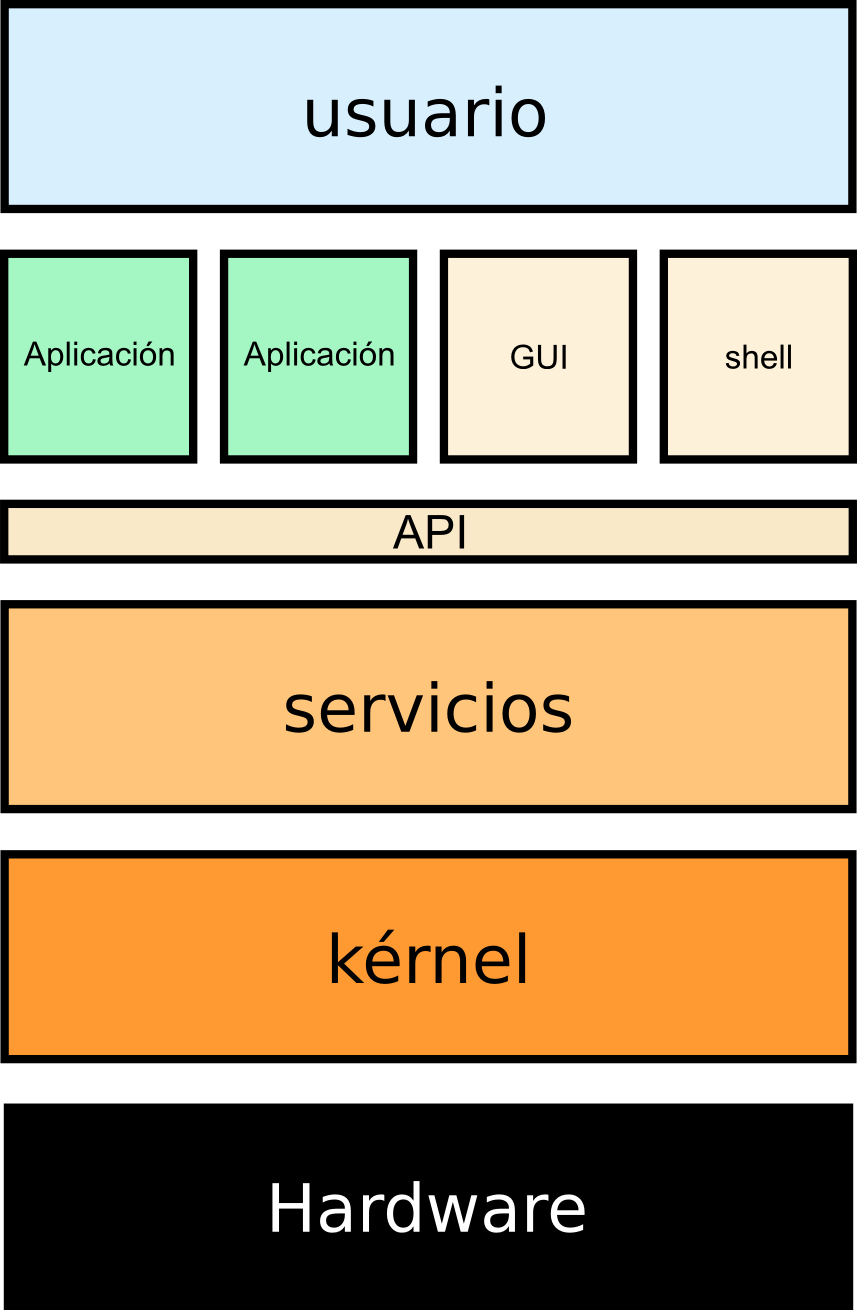
\includegraphics[width=\columnwidth]{img/SO.png}    
    \end{center}
  \end{columns}
\end{frame}

\begin{frame}
  \frametitle{¿GUI, CLI o ambas?}
  \begin{center}
    \begin{block}{GUI}
      \begin{itemize}
      \item Más sencilla inicialmente
      \item Útil para usuarios finales
      \item No programable
      \item Para equipos locales
      \end{itemize}
    \end{block}
    \begin{block}{CLI}
      \begin{itemize}
      \item Más compleja inicialmente
      \item Útil para usuarios avanzados
      \item Programable
      \item Para equipos locales o remotos
      \end{itemize}
    \end{block}
  \end{center}

\end{frame}

\begin{frame}
  \frametitle{Sistemas tipo UNIX}
  \begin{center}
    \begin{itemize}
    \item Unics: Creado en 1969 por Thompson y Ritchie de Bell Labs en
      ensamblador, basándose en el sistema Multics
    \item Renombrado posteriormente a Unix
    \item Reescrito casi completamente en C en 1973 
    \item Principales características:
      \begin{itemize}
      \item Multitarea
      \item Multiusuario
      \item Portable
      \end{itemize}
    \item Familias UNIX
      \begin{itemize}
      \item BSD (FreeBSD, OpenBSD, Mac OS X, \ldots)
      \item System V (AIX, \sout{XeniX}, Solaris, HP-UX)
      \item Minix
      \item Linux
      \end{itemize}
    \item UNIX{\textregistered} y los litigios por el nombre
    \item POSIX (Portable Operating System Interface)
    \end{itemize}
  \end{center}
\end{frame}

\begin{frame}
  \frametitle{Más de 50 años de Unix}
  \begin{center}
    \begin{itemize}
    \item Sistema inicialmente pensado para el entorno profesional
    \item La portabilidad de Unix ha permitido adaptarlo a gran cantidad de
      microarquitecturas.
    \item Unix y el software libre (*BSD, GNU/Linux y OpenSolaris)
    \item Sí. Seguramente llevas un Unix en el bolsillo ;-)
    \item Filosofía UNIX:
      \begin{itemize}
      \item Lo pequeño es hermoso
      \item Haz que cada programa haga una cosa bien
      \item Construye un prototipo lo antes posible
      \item Elige portabilidad sobre eficiencia
      \item Guarda los datos en archivos de texto plano
      \item Aprovecha funcionalidades del software
      \item Usa shell scripts para aumentar la funcionalidad y portabilidad
      \item \ldots
      \end{itemize}
    \end{itemize}
  \end{center}
\end{frame}

\begin{frame} \frametitle{Historia de UNIX}
  \begin{center}
    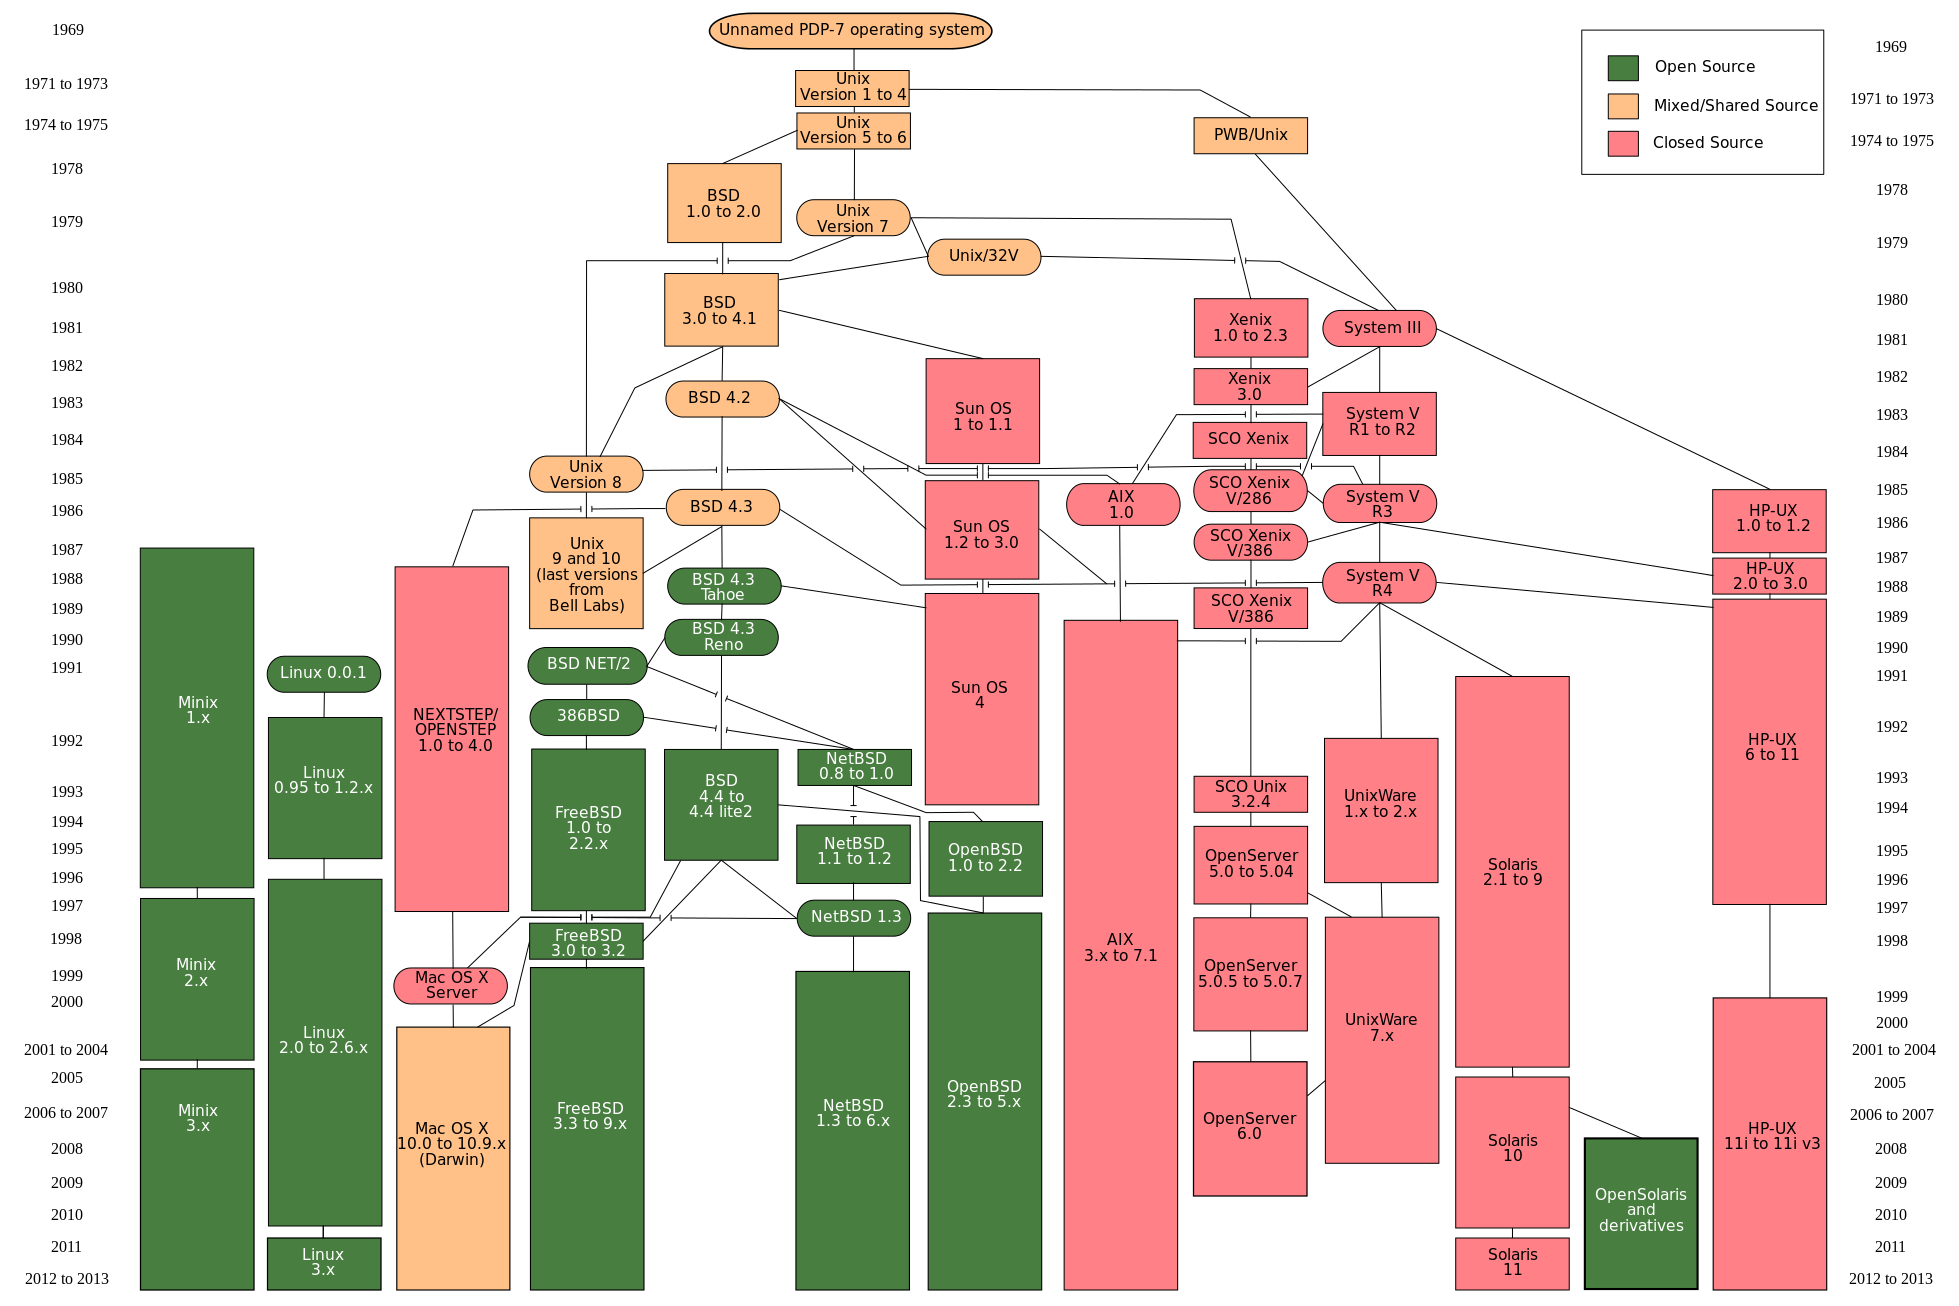
\includegraphics[width=.85\textwidth]{img/Unix_history-simple.png}
\end{center}\tiny{Fuente: \url{http://upload.wikimedia.org/wikipedia/commons/5/50/Unix_history-simple.png}}
\end{frame}

\begin{frame}
  \frametitle{Ms Windows}
  \begin{center}
    \begin{itemize}
    \item Sistemas operativos para IBM-PC y compatibles con microprocesadores
      x86
    \item Wintel: Windows + Intel
    \item Informática doméstica
    \item Comenzaron con una interfaz gráfica (GUI) para Ms-DOS
    \item 1985-1990 Versiones 1.0 y 2.0
    \item 1991-1992 Windows 3.0 y sobre todo Windows 3.1 comienzan a utilizarse por el
      gran público
    \item Bill Gates: ``Internet no tiene futuro''
    \item Windows 95, Windows 98 y \sout{Windows ME} y la popularidad de los
      PC.
    \item \textbf{Era PC} en el hogar. 
    \end{itemize}
  \end{center}
\end{frame}

\begin{frame}
  \frametitle{Ms Windows. Familia NT}
    \begin{itemize}
    \item Desarrollo nuevo e independiente a partir de 1993
    \item Principales características:
      \begin{itemize}
      \item Multitarea
      \item Multiusuario
      \item Portable
      \end{itemize}
    \item Sistemas NT orientados inicialmente para la informática empresarial
    \item NT 3.1 (1993), NT 4 (1996)
    \item \textbf{Era PC} en la empresa: Se sustituyen sistemas centralizados
      por equipos pequeños autónomos.
    \item Windows 20XX triunfa en la Intranet
    \item Windows XP: el primer sistema para millones de personas
    \item Windows Vista, 7, 8, 10, \ldots
    \item ¿Estamos ya en la \textbf{Era Post-PC}?
    \end{itemize}
\end{frame}

\begin{frame}
  \frametitle{Apple}
    \begin{itemize}
    \item 1984: Apple Macinstosh (Mac) con interfaz gráfica para el usuario
      doméstico.
    \item Hardware + software
    \item Inicialmente utilizaban procesadores Motorola 68000
    \item Mac OS System 1-7
    \item Años 90: Se comienzan a utilizar los potentes procesadores powerpc de
      IBM.
    \item Apple triunfa en algunos nichos de mercado pero fracasa entre el gran
      público. Mac OS 8-9
    \item Mac OS X con procesadores Intel x86\_64. Sistema tipo UNIX no compatible
      con equipos anteriores
    \item iOS e iPadOS
    \end{itemize}
\end{frame}

\begin{frame}
  \frametitle{GNU/Linux}
  \begin{itemize}
  \item 1991: GNU de la FSF + kérnel linux sobre x86
  \item Sistema tipo UNIX (compatible POSIX)
  \item Software libre
  \item Distribuido inicialmente entre aficionados
  \item Distribuciones
  \item Va aglutinando comunidades de software libre y empresas
  \item Se porta a más de 20 microarquitecturas
  \item Amplio espectro: desde equipos empotrados a grandes superordenadores
  \item Triunfa en todos los sectores salvo en el escritorio
  \item Este año va a ser el de linux en el escritorio ¡ejem!    
  \end{itemize}
\end{frame}

\begin{frame} \frametitle{Sistemas operativos para móviles}
  \begin{center}
    \begin{tabular}[center]{|l|ccc|}
      \hline
      Nombre & Creador & Basado en& Licencia\\
      \hline
      Android&Google&GNU/Linux&\sout{Libre}\\
      iOS&Apple&OS X&Privativa\\
      iPadOS&Apple&OS X&Privativa\\
      Windows 10&Microsoft&&Privativa\\
      Chrome OS&Google&GNU/Linux&\sout{Libre}\\
      Tizen&Samsung&GNU/Linux&\sout{Libre}\\
      LineageOS&Comunidad&GNU/Linux&Libre\\
      PureOS&Purism&GNU/Linux&Libre\\
      Ubuntu Touch&UBports&GNU/Linux&Libre\\
      {\color{red}Symbian}&Nokia&&Privativa\\
      {\color{red}Blackberry OS}&RIM&&Privativa\\
      {\color{red}Windows Mobile}&Microsoft&Windows CE&Privativa\\
      \hline
    \end{tabular}
  \end{center}

    Cyanogenmod, MeeGo/Maemo/Moblin, Firefox OS, webOS, Bada, Palm OS, etc.   
\end{frame}

\begin{frame} \frametitle{Uso de sistemas operativos móviles}
  \begin{center}
    \url{https://gs.statcounter.com/os-market-share/mobile/worldwide}
\end{center}
\end{frame}

\begin{frame} \frametitle{Sistemas operativos. Servidores}
  \begin{center}
    \begin{tabular}[center]{|l|ccc|}
      \hline
      Nombre & Creador & Basado en& Licencia\\
      \hline
      AIX & IBM & System-V & Privativa\\
      HP-UX & HP & Unix & Privativa\\
      GNU/Linux & Comunidad & Unix & GPL\\
      Solaris&\sout{Sun} Oracle& Unix & Privativa\\
      OpenSolaris & \sout{Sun} Oracle & Solaris & CDDL\\
      FreeBSD & Comunidad & 386BSD & BSD\\
      OpenBSD & Comunidad & 386BSD & BSD\\
      Windows server & Microsoft & & Privativa\\
      z/OS & IBM & OS/390 & Privativa\\
      \hline
    \end{tabular}
  \end{center}
\tiny{Fuente: \url{http://en.wikipedia.org/wiki/Comparison_of_operating_systems}}
\end{frame}

\begin{frame}
  \frametitle{El sorpasso}
 Windows parece que ya no es el principal sistema operativo en los clientes\par
 \begin{itemize}
  \item \href{http://gs.statcounter.com/os-market-share\#monthly-200901-202009}{statcounter 2009-2020}
 \item \href{https://en.wikipedia.org/wiki/Usage\_share\_of\_operating\_systems}{Wikipedia - Usage share operating systems}
 \item \href{https://bugs.launchpad.net/ubuntu/+bug/1}{Ubuntu Bug nº1}
 \end{itemize}
\end{frame}

\begin{frame}
  \frametitle{Linux ganó}
  El kérnel linux es el más utilizado en los diferentes sistemas
  operativos de \textbf{todos} los segmentos de ordenadores hoy en
  día:
  \begin{itemize}
  \item Supercomputadoras \href{https://www.top500.org/statistics/details/osfam/1}{top 500}
  \item Servidores en centros de datos
  \item Equipos clientes (android)
  \item Sistemas empotrados
  \end{itemize}
  Aunque eso no significa siempre que ganase el software libre :-/
\end{frame}

\end{document}